% Options for packages loaded elsewhere
\PassOptionsToPackage{unicode}{hyperref}
\PassOptionsToPackage{hyphens}{url}
\PassOptionsToPackage{dvipsnames,svgnames,x11names}{xcolor}
%
\documentclass[
  letterpaper,
  DIV=11,
  numbers=noendperiod]{scrartcl}

\usepackage{amsmath,amssymb}
\usepackage{iftex}
\ifPDFTeX
  \usepackage[T1]{fontenc}
  \usepackage[utf8]{inputenc}
  \usepackage{textcomp} % provide euro and other symbols
\else % if luatex or xetex
  \usepackage{unicode-math}
  \defaultfontfeatures{Scale=MatchLowercase}
  \defaultfontfeatures[\rmfamily]{Ligatures=TeX,Scale=1}
\fi
\usepackage{lmodern}
\ifPDFTeX\else  
    % xetex/luatex font selection
\fi
% Use upquote if available, for straight quotes in verbatim environments
\IfFileExists{upquote.sty}{\usepackage{upquote}}{}
\IfFileExists{microtype.sty}{% use microtype if available
  \usepackage[]{microtype}
  \UseMicrotypeSet[protrusion]{basicmath} % disable protrusion for tt fonts
}{}
\makeatletter
\@ifundefined{KOMAClassName}{% if non-KOMA class
  \IfFileExists{parskip.sty}{%
    \usepackage{parskip}
  }{% else
    \setlength{\parindent}{0pt}
    \setlength{\parskip}{6pt plus 2pt minus 1pt}}
}{% if KOMA class
  \KOMAoptions{parskip=half}}
\makeatother
\usepackage{xcolor}
\setlength{\emergencystretch}{3em} % prevent overfull lines
\setcounter{secnumdepth}{-\maxdimen} % remove section numbering
% Make \paragraph and \subparagraph free-standing
\ifx\paragraph\undefined\else
  \let\oldparagraph\paragraph
  \renewcommand{\paragraph}[1]{\oldparagraph{#1}\mbox{}}
\fi
\ifx\subparagraph\undefined\else
  \let\oldsubparagraph\subparagraph
  \renewcommand{\subparagraph}[1]{\oldsubparagraph{#1}\mbox{}}
\fi

\usepackage{color}
\usepackage{fancyvrb}
\newcommand{\VerbBar}{|}
\newcommand{\VERB}{\Verb[commandchars=\\\{\}]}
\DefineVerbatimEnvironment{Highlighting}{Verbatim}{commandchars=\\\{\}}
% Add ',fontsize=\small' for more characters per line
\usepackage{framed}
\definecolor{shadecolor}{RGB}{241,243,245}
\newenvironment{Shaded}{\begin{snugshade}}{\end{snugshade}}
\newcommand{\AlertTok}[1]{\textcolor[rgb]{0.68,0.00,0.00}{#1}}
\newcommand{\AnnotationTok}[1]{\textcolor[rgb]{0.37,0.37,0.37}{#1}}
\newcommand{\AttributeTok}[1]{\textcolor[rgb]{0.40,0.45,0.13}{#1}}
\newcommand{\BaseNTok}[1]{\textcolor[rgb]{0.68,0.00,0.00}{#1}}
\newcommand{\BuiltInTok}[1]{\textcolor[rgb]{0.00,0.23,0.31}{#1}}
\newcommand{\CharTok}[1]{\textcolor[rgb]{0.13,0.47,0.30}{#1}}
\newcommand{\CommentTok}[1]{\textcolor[rgb]{0.37,0.37,0.37}{#1}}
\newcommand{\CommentVarTok}[1]{\textcolor[rgb]{0.37,0.37,0.37}{\textit{#1}}}
\newcommand{\ConstantTok}[1]{\textcolor[rgb]{0.56,0.35,0.01}{#1}}
\newcommand{\ControlFlowTok}[1]{\textcolor[rgb]{0.00,0.23,0.31}{#1}}
\newcommand{\DataTypeTok}[1]{\textcolor[rgb]{0.68,0.00,0.00}{#1}}
\newcommand{\DecValTok}[1]{\textcolor[rgb]{0.68,0.00,0.00}{#1}}
\newcommand{\DocumentationTok}[1]{\textcolor[rgb]{0.37,0.37,0.37}{\textit{#1}}}
\newcommand{\ErrorTok}[1]{\textcolor[rgb]{0.68,0.00,0.00}{#1}}
\newcommand{\ExtensionTok}[1]{\textcolor[rgb]{0.00,0.23,0.31}{#1}}
\newcommand{\FloatTok}[1]{\textcolor[rgb]{0.68,0.00,0.00}{#1}}
\newcommand{\FunctionTok}[1]{\textcolor[rgb]{0.28,0.35,0.67}{#1}}
\newcommand{\ImportTok}[1]{\textcolor[rgb]{0.00,0.46,0.62}{#1}}
\newcommand{\InformationTok}[1]{\textcolor[rgb]{0.37,0.37,0.37}{#1}}
\newcommand{\KeywordTok}[1]{\textcolor[rgb]{0.00,0.23,0.31}{#1}}
\newcommand{\NormalTok}[1]{\textcolor[rgb]{0.00,0.23,0.31}{#1}}
\newcommand{\OperatorTok}[1]{\textcolor[rgb]{0.37,0.37,0.37}{#1}}
\newcommand{\OtherTok}[1]{\textcolor[rgb]{0.00,0.23,0.31}{#1}}
\newcommand{\PreprocessorTok}[1]{\textcolor[rgb]{0.68,0.00,0.00}{#1}}
\newcommand{\RegionMarkerTok}[1]{\textcolor[rgb]{0.00,0.23,0.31}{#1}}
\newcommand{\SpecialCharTok}[1]{\textcolor[rgb]{0.37,0.37,0.37}{#1}}
\newcommand{\SpecialStringTok}[1]{\textcolor[rgb]{0.13,0.47,0.30}{#1}}
\newcommand{\StringTok}[1]{\textcolor[rgb]{0.13,0.47,0.30}{#1}}
\newcommand{\VariableTok}[1]{\textcolor[rgb]{0.07,0.07,0.07}{#1}}
\newcommand{\VerbatimStringTok}[1]{\textcolor[rgb]{0.13,0.47,0.30}{#1}}
\newcommand{\WarningTok}[1]{\textcolor[rgb]{0.37,0.37,0.37}{\textit{#1}}}

\providecommand{\tightlist}{%
  \setlength{\itemsep}{0pt}\setlength{\parskip}{0pt}}\usepackage{longtable,booktabs,array}
\usepackage{calc} % for calculating minipage widths
% Correct order of tables after \paragraph or \subparagraph
\usepackage{etoolbox}
\makeatletter
\patchcmd\longtable{\par}{\if@noskipsec\mbox{}\fi\par}{}{}
\makeatother
% Allow footnotes in longtable head/foot
\IfFileExists{footnotehyper.sty}{\usepackage{footnotehyper}}{\usepackage{footnote}}
\makesavenoteenv{longtable}
\usepackage{graphicx}
\makeatletter
\def\maxwidth{\ifdim\Gin@nat@width>\linewidth\linewidth\else\Gin@nat@width\fi}
\def\maxheight{\ifdim\Gin@nat@height>\textheight\textheight\else\Gin@nat@height\fi}
\makeatother
% Scale images if necessary, so that they will not overflow the page
% margins by default, and it is still possible to overwrite the defaults
% using explicit options in \includegraphics[width, height, ...]{}
\setkeys{Gin}{width=\maxwidth,height=\maxheight,keepaspectratio}
% Set default figure placement to htbp
\makeatletter
\def\fps@figure{htbp}
\makeatother

\KOMAoption{captions}{tableheading}
\makeatletter
\makeatother
\makeatletter
\makeatother
\makeatletter
\@ifpackageloaded{caption}{}{\usepackage{caption}}
\AtBeginDocument{%
\ifdefined\contentsname
  \renewcommand*\contentsname{Table of contents}
\else
  \newcommand\contentsname{Table of contents}
\fi
\ifdefined\listfigurename
  \renewcommand*\listfigurename{List of Figures}
\else
  \newcommand\listfigurename{List of Figures}
\fi
\ifdefined\listtablename
  \renewcommand*\listtablename{List of Tables}
\else
  \newcommand\listtablename{List of Tables}
\fi
\ifdefined\figurename
  \renewcommand*\figurename{Figure}
\else
  \newcommand\figurename{Figure}
\fi
\ifdefined\tablename
  \renewcommand*\tablename{Table}
\else
  \newcommand\tablename{Table}
\fi
}
\@ifpackageloaded{float}{}{\usepackage{float}}
\floatstyle{ruled}
\@ifundefined{c@chapter}{\newfloat{codelisting}{h}{lop}}{\newfloat{codelisting}{h}{lop}[chapter]}
\floatname{codelisting}{Listing}
\newcommand*\listoflistings{\listof{codelisting}{List of Listings}}
\makeatother
\makeatletter
\@ifpackageloaded{caption}{}{\usepackage{caption}}
\@ifpackageloaded{subcaption}{}{\usepackage{subcaption}}
\makeatother
\makeatletter
\@ifpackageloaded{tcolorbox}{}{\usepackage[skins,breakable]{tcolorbox}}
\makeatother
\makeatletter
\@ifundefined{shadecolor}{\definecolor{shadecolor}{rgb}{.97, .97, .97}}
\makeatother
\makeatletter
\makeatother
\makeatletter
\makeatother
\ifLuaTeX
  \usepackage{selnolig}  % disable illegal ligatures
\fi
\IfFileExists{bookmark.sty}{\usepackage{bookmark}}{\usepackage{hyperref}}
\IfFileExists{xurl.sty}{\usepackage{xurl}}{} % add URL line breaks if available
\urlstyle{same} % disable monospaced font for URLs
\hypersetup{
  pdftitle={Exercise 2},
  pdfauthor={Joaquin Ramirez},
  colorlinks=true,
  linkcolor={blue},
  filecolor={Maroon},
  citecolor={Blue},
  urlcolor={Blue},
  pdfcreator={LaTeX via pandoc}}

\title{Exercise 2}
\author{Joaquin Ramirez}
\date{}

\begin{document}
\maketitle
\ifdefined\Shaded\renewenvironment{Shaded}{\begin{tcolorbox}[enhanced, breakable, sharp corners, interior hidden, boxrule=0pt, borderline west={3pt}{0pt}{shadecolor}, frame hidden]}{\end{tcolorbox}}\fi

\begin{Shaded}
\begin{Highlighting}[]
\CommentTok{\#install.packages(\textquotesingle{}mlbench\textquotesingle{})}
\CommentTok{\#install.packages(\textquotesingle{}ggplot2\textquotesingle{})}
\CommentTok{\#install.packages(\textquotesingle{}GGally\textquotesingle{})}
\CommentTok{\#install.packages(\textquotesingle{}corrplot\textquotesingle{})}
\CommentTok{\#install.packages(\textquotesingle{}gridExtra\textquotesingle{})}
\CommentTok{\#install.packages(\textquotesingle{}kernlab\textquotesingle{})}
\FunctionTok{library}\NormalTok{(kernlab) }
\FunctionTok{library}\NormalTok{(mlbench)}
\end{Highlighting}
\end{Shaded}

\begin{verbatim}
Warning: package 'mlbench' was built under R version 4.3.3
\end{verbatim}

\begin{Shaded}
\begin{Highlighting}[]
\FunctionTok{library}\NormalTok{(ggplot2)}
\end{Highlighting}
\end{Shaded}

\begin{verbatim}
Warning: package 'ggplot2' was built under R version 4.3.2
\end{verbatim}

\begin{verbatim}

Attaching package: 'ggplot2'
\end{verbatim}

\begin{verbatim}
The following object is masked from 'package:kernlab':

    alpha
\end{verbatim}

\begin{Shaded}
\begin{Highlighting}[]
\FunctionTok{library}\NormalTok{(GGally)}
\end{Highlighting}
\end{Shaded}

\begin{verbatim}
Warning: package 'GGally' was built under R version 4.3.3
\end{verbatim}

\begin{verbatim}
Registered S3 method overwritten by 'GGally':
  method from   
  +.gg   ggplot2
\end{verbatim}

\begin{Shaded}
\begin{Highlighting}[]
\FunctionTok{library}\NormalTok{(corrplot)}
\end{Highlighting}
\end{Shaded}

\begin{verbatim}
Warning: package 'corrplot' was built under R version 4.3.3
\end{verbatim}

\begin{verbatim}
corrplot 0.92 loaded
\end{verbatim}

\begin{Shaded}
\begin{Highlighting}[]
\FunctionTok{library}\NormalTok{(gridExtra)}
\FunctionTok{library}\NormalTok{(AppliedPredictiveModeling)}
\end{Highlighting}
\end{Shaded}

\begin{verbatim}
Warning: package 'AppliedPredictiveModeling' was built under R version 4.3.3
\end{verbatim}

\begin{Shaded}
\begin{Highlighting}[]
\FunctionTok{library}\NormalTok{(caret)}
\end{Highlighting}
\end{Shaded}

\begin{verbatim}
Warning: package 'caret' was built under R version 4.3.3
\end{verbatim}

\begin{verbatim}
Loading required package: lattice
\end{verbatim}

The UC Irvine Machine Learning Repository contains a data set related to
glass identification. The data consists of 214 glass samples labeled as
one of seven class categories. There are nine predictors, including the
refractive index and percentages of eight elements: Na, Mg, Al, Si, K,
Ca, Ba, and Fe.

The data can be accessed via

\begin{Shaded}
\begin{Highlighting}[]
\FunctionTok{data}\NormalTok{(Glass)}
\FunctionTok{str}\NormalTok{(Glass)}
\end{Highlighting}
\end{Shaded}

\begin{verbatim}
'data.frame':   214 obs. of  10 variables:
 $ RI  : num  1.52 1.52 1.52 1.52 1.52 ...
 $ Na  : num  13.6 13.9 13.5 13.2 13.3 ...
 $ Mg  : num  4.49 3.6 3.55 3.69 3.62 3.61 3.6 3.61 3.58 3.6 ...
 $ Al  : num  1.1 1.36 1.54 1.29 1.24 1.62 1.14 1.05 1.37 1.36 ...
 $ Si  : num  71.8 72.7 73 72.6 73.1 ...
 $ K   : num  0.06 0.48 0.39 0.57 0.55 0.64 0.58 0.57 0.56 0.57 ...
 $ Ca  : num  8.75 7.83 7.78 8.22 8.07 8.07 8.17 8.24 8.3 8.4 ...
 $ Ba  : num  0 0 0 0 0 0 0 0 0 0 ...
 $ Fe  : num  0 0 0 0 0 0.26 0 0 0 0.11 ...
 $ Type: Factor w/ 6 levels "1","2","3","5",..: 1 1 1 1 1 1 1 1 1 1 ...
\end{verbatim}

\textbf{a) Utilize suitable visualizations (employ any types of data
visualization you deem appropriate) to explore the predictor variables,
aiming to understand their distributions and relationships among them.}

\textbf{Boxplots:}

\begin{Shaded}
\begin{Highlighting}[]
\FunctionTok{data}\NormalTok{(Glass)}
\NormalTok{Glass}\SpecialCharTok{$}\NormalTok{Type }\OtherTok{\textless{}{-}} \FunctionTok{as.factor}\NormalTok{(Glass}\SpecialCharTok{$}\NormalTok{Type)}

\NormalTok{boxplots }\OtherTok{\textless{}{-}} \FunctionTok{lapply}\NormalTok{(}\FunctionTok{names}\NormalTok{(Glass)[}\DecValTok{1}\SpecialCharTok{:}\DecValTok{9}\NormalTok{], }\ControlFlowTok{function}\NormalTok{(var) \{}\FunctionTok{ggplot}\NormalTok{(Glass, }\FunctionTok{aes\_string}\NormalTok{(}\AttributeTok{x =} \StringTok{"Type"}\NormalTok{, }\AttributeTok{y =}\NormalTok{ var)) }\SpecialCharTok{+} 
    \FunctionTok{geom\_boxplot}\NormalTok{() }\SpecialCharTok{+} 
    \FunctionTok{ggtitle}\NormalTok{(}\FunctionTok{paste}\NormalTok{(}\StringTok{"Boxplot of"}\NormalTok{, var)) }\SpecialCharTok{+} 
    \FunctionTok{theme\_minimal}\NormalTok{() }\SpecialCharTok{+}
    \FunctionTok{theme\_dark}\NormalTok{()\})}
\end{Highlighting}
\end{Shaded}

\begin{verbatim}
Warning: `aes_string()` was deprecated in ggplot2 3.0.0.
i Please use tidy evaluation idioms with `aes()`.
i See also `vignette("ggplot2-in-packages")` for more information.
\end{verbatim}

\begin{Shaded}
\begin{Highlighting}[]
\NormalTok{boxplots\_combined }\OtherTok{\textless{}{-}} \FunctionTok{do.call}\NormalTok{(grid.arrange, }\FunctionTok{c}\NormalTok{(boxplots, }\AttributeTok{ncol =} \DecValTok{3}\NormalTok{))}
\end{Highlighting}
\end{Shaded}

\begin{figure}[H]

{\centering 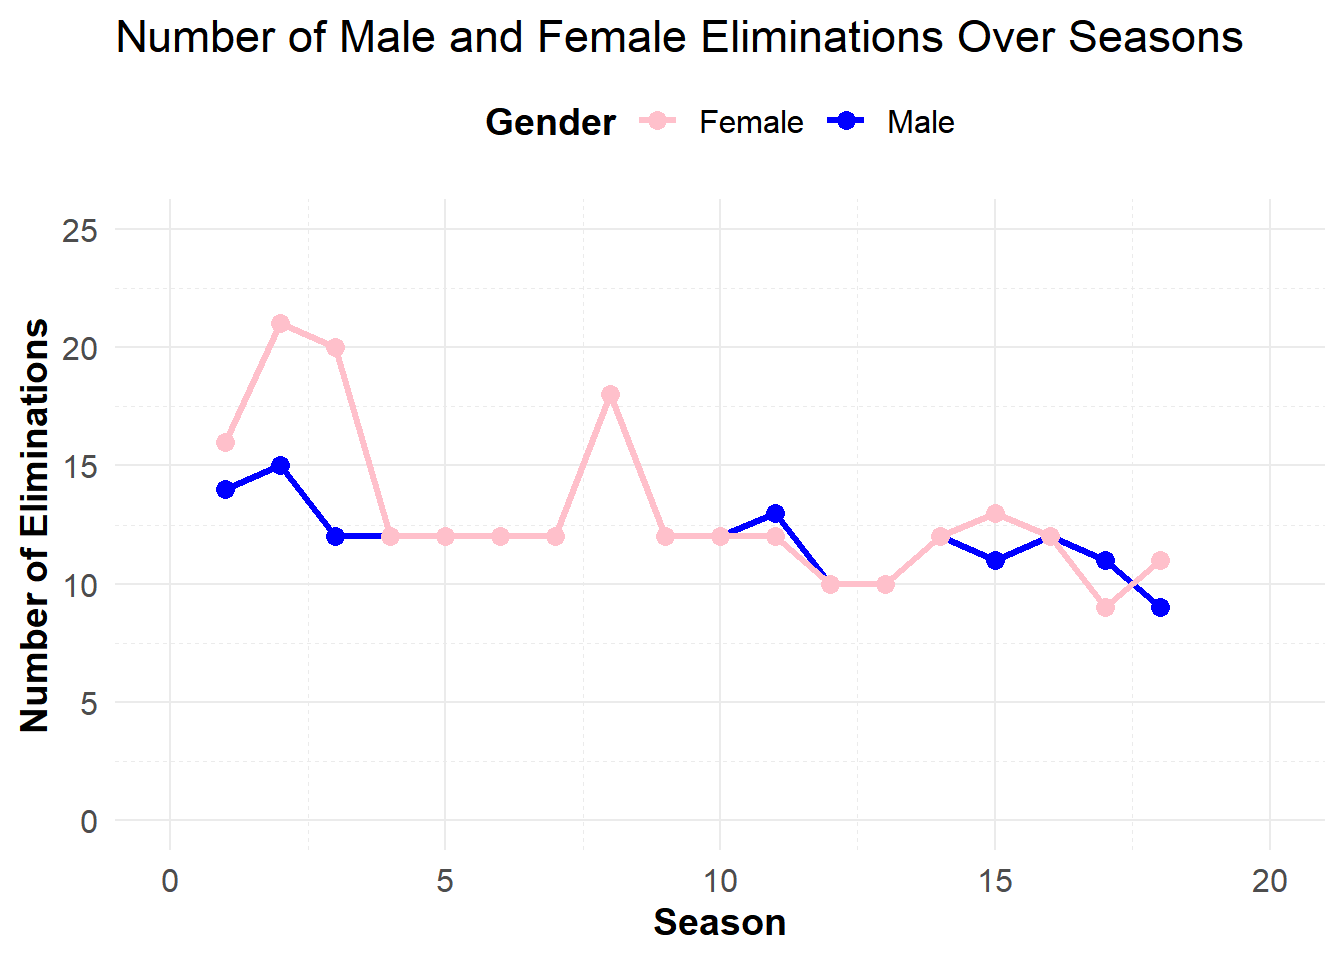
\includegraphics{Exercise-2_files/figure-pdf/unnamed-chunk-3-1.pdf}

}

\end{figure}

\textbf{Histograms:}

\begin{Shaded}
\begin{Highlighting}[]
\NormalTok{histograms }\OtherTok{\textless{}{-}} \FunctionTok{lapply}\NormalTok{(}\FunctionTok{names}\NormalTok{(Glass)[}\DecValTok{1}\SpecialCharTok{:}\DecValTok{9}\NormalTok{], }\ControlFlowTok{function}\NormalTok{(var) \{}\FunctionTok{ggplot}\NormalTok{(Glass, }\FunctionTok{aes\_string}\NormalTok{(}\AttributeTok{x =}\NormalTok{ var)) }\SpecialCharTok{+} 
    \FunctionTok{geom\_histogram}\NormalTok{(}\AttributeTok{bins =} \DecValTok{30}\NormalTok{) }\SpecialCharTok{+} 
    \FunctionTok{ggtitle}\NormalTok{(}\FunctionTok{paste}\NormalTok{(}\StringTok{"Histogram of"}\NormalTok{, var)) }\SpecialCharTok{+} 
    \FunctionTok{theme\_minimal}\NormalTok{() }\SpecialCharTok{+}
    \FunctionTok{theme\_classic}\NormalTok{()\})}


\NormalTok{histogram\_combined }\OtherTok{\textless{}{-}} \FunctionTok{do.call}\NormalTok{(grid.arrange, }\FunctionTok{c}\NormalTok{(histograms, }\AttributeTok{ncol =} \DecValTok{3}\NormalTok{))}
\end{Highlighting}
\end{Shaded}

\begin{figure}[H]

{\centering 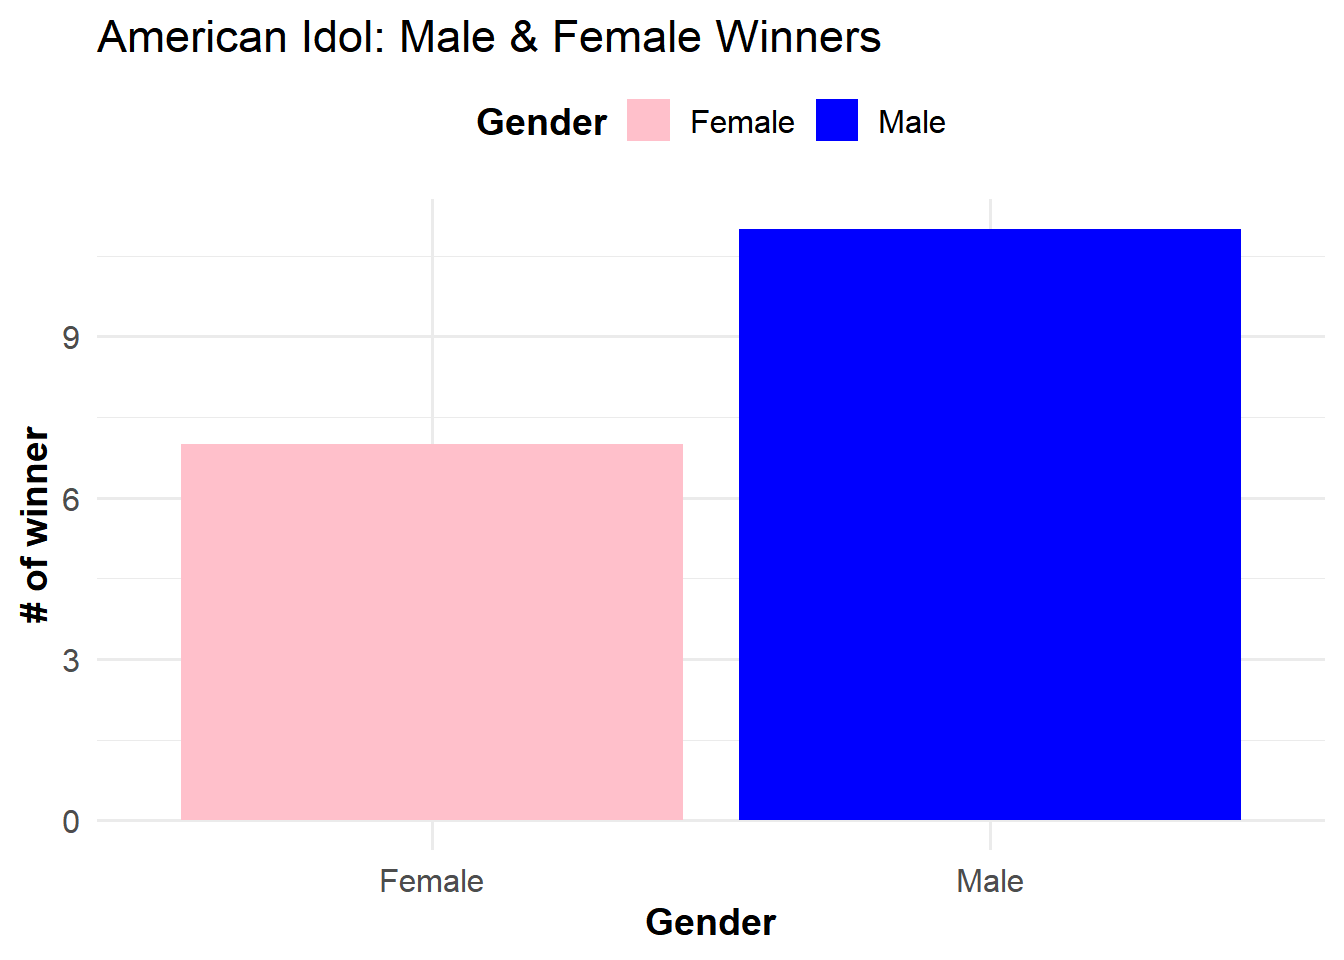
\includegraphics{Exercise-2_files/figure-pdf/unnamed-chunk-4-1.pdf}

}

\end{figure}

I utilized both Histograms and Boxplots, you can definitely see a lot of
outliers in the plots displayed. Na and Al, seem to be normally
distributed but all other seem to be either skewed to the left or to the
right.

\textbf{b) Do there appear to be any outliers in the data? Are any
predictors skewed? Show all the work! }

\begin{itemize}
\tightlist
\item
  Function to create boxplots for each predictor:
\end{itemize}

\begin{Shaded}
\begin{Highlighting}[]
\NormalTok{create\_boxplot }\OtherTok{\textless{}{-}} \ControlFlowTok{function}\NormalTok{(data, var) \{}
  \FunctionTok{ggplot}\NormalTok{(data, }\FunctionTok{aes\_string}\NormalTok{(}\AttributeTok{y =}\NormalTok{ var)) }\SpecialCharTok{+} 
    \FunctionTok{geom\_boxplot}\NormalTok{() }\SpecialCharTok{+} 
    \FunctionTok{ggtitle}\NormalTok{(}\FunctionTok{paste}\NormalTok{(}\StringTok{"Boxplot of"}\NormalTok{, var)) }\SpecialCharTok{+} 
    \FunctionTok{theme\_minimal}\NormalTok{() }\SpecialCharTok{+}
    \FunctionTok{theme\_classic}\NormalTok{()\}}


\NormalTok{boxplots }\OtherTok{\textless{}{-}} \FunctionTok{lapply}\NormalTok{(}\FunctionTok{names}\NormalTok{(Glass)[}\DecValTok{1}\SpecialCharTok{:}\DecValTok{9}\NormalTok{], }\ControlFlowTok{function}\NormalTok{(var) }\FunctionTok{create\_boxplot}\NormalTok{(Glass, var))}
\FunctionTok{do.call}\NormalTok{(grid.arrange, }\FunctionTok{c}\NormalTok{(boxplots, }\AttributeTok{ncol =} \DecValTok{3}\NormalTok{))}
\end{Highlighting}
\end{Shaded}

\begin{figure}[H]

{\centering 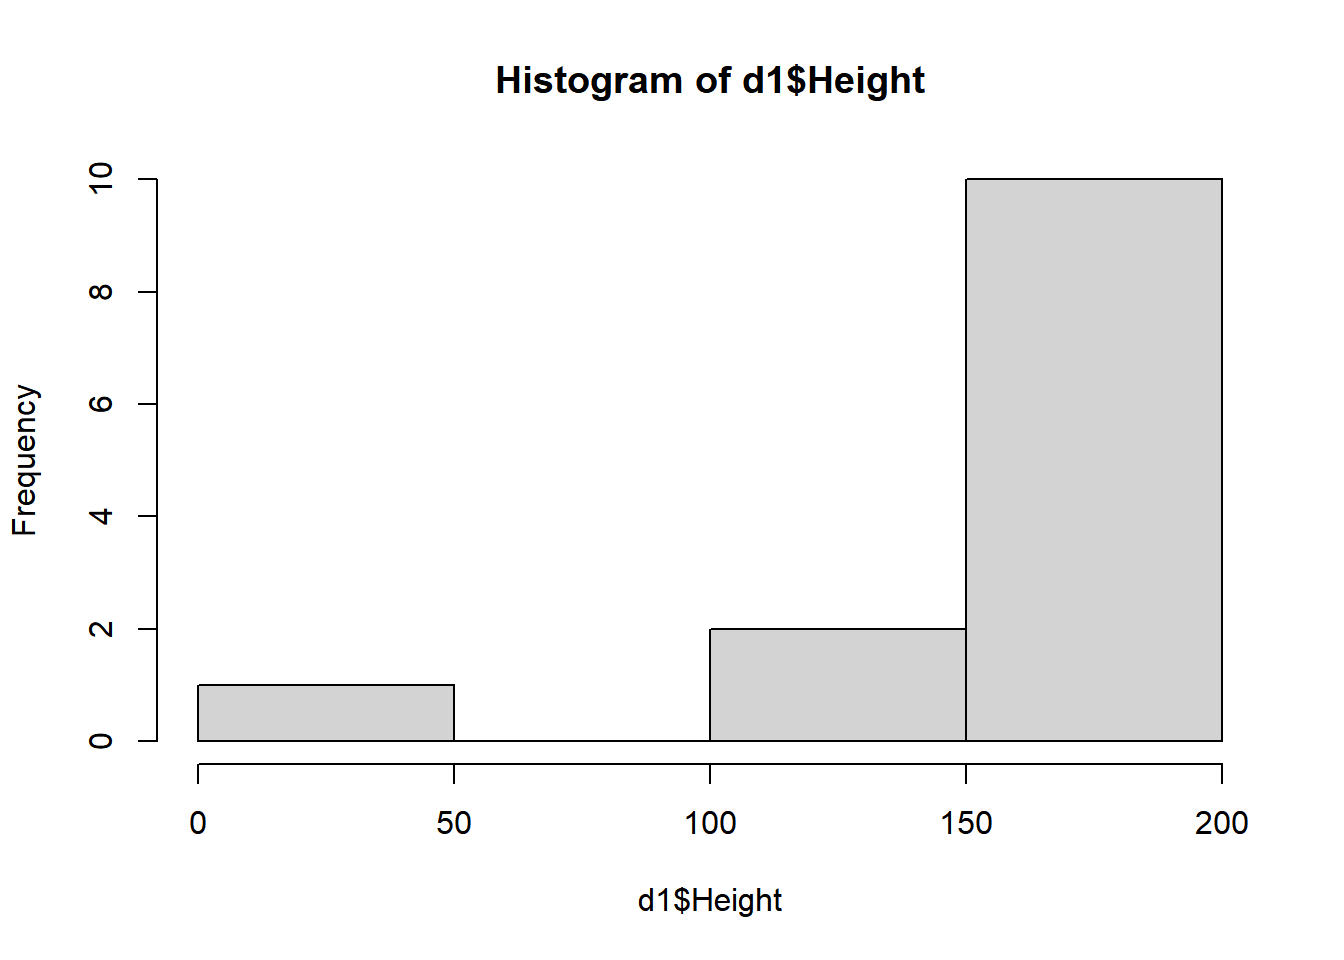
\includegraphics{Exercise-2_files/figure-pdf/unnamed-chunk-5-1.pdf}

}

\end{figure}

Predictors Outliers from Boxplots:

\begin{itemize}
\item
  RI (Refractive Index): Significant outliers exist
\item
  Na (Sodium): Fewer outliers exist, with some extreme values
\item
  Mg (Magnesium): No outliers
\item
  Al (Aluminum): Significant Outliers exist, with extreme values
\item
  Si (Silicon): Significant outliers exist, with extreme values
\item
  K (Potassium): Outliers exist, fewer extreme values
\item
  Ca (Calcium): Significant outliers are existing.
\item
  Ba (Barium): Significant outliers observed, with many extreme value
\item
  Fe (Iron): Outliers observed with few extreme values
\item
  Function to create histograms for each predictor
\end{itemize}

\begin{Shaded}
\begin{Highlighting}[]
\NormalTok{create\_histogram }\OtherTok{\textless{}{-}} \ControlFlowTok{function}\NormalTok{(data, var) \{}
  \FunctionTok{ggplot}\NormalTok{(data, }\FunctionTok{aes\_string}\NormalTok{(}\AttributeTok{x =}\NormalTok{ var)) }\SpecialCharTok{+} 
    \FunctionTok{geom\_histogram}\NormalTok{(}\AttributeTok{bins =} \DecValTok{30}\NormalTok{) }\SpecialCharTok{+} 
    \FunctionTok{ggtitle}\NormalTok{(}\FunctionTok{paste}\NormalTok{(}\StringTok{"Histogram of"}\NormalTok{, var)) }\SpecialCharTok{+} 
    \FunctionTok{theme\_minimal}\NormalTok{() }\SpecialCharTok{+}
    \FunctionTok{theme\_classic}\NormalTok{()\}}


\NormalTok{histograms }\OtherTok{\textless{}{-}} \FunctionTok{lapply}\NormalTok{(}\FunctionTok{names}\NormalTok{(Glass)[}\DecValTok{1}\SpecialCharTok{:}\DecValTok{9}\NormalTok{], }\ControlFlowTok{function}\NormalTok{(var) }\FunctionTok{create\_histogram}\NormalTok{(Glass, var))}
\NormalTok{histo }\OtherTok{\textless{}{-}} \FunctionTok{do.call}\NormalTok{(grid.arrange, }\FunctionTok{c}\NormalTok{(histograms, }\AttributeTok{ncol =} \DecValTok{3}\NormalTok{))}
\end{Highlighting}
\end{Shaded}

\begin{figure}[H]

{\centering 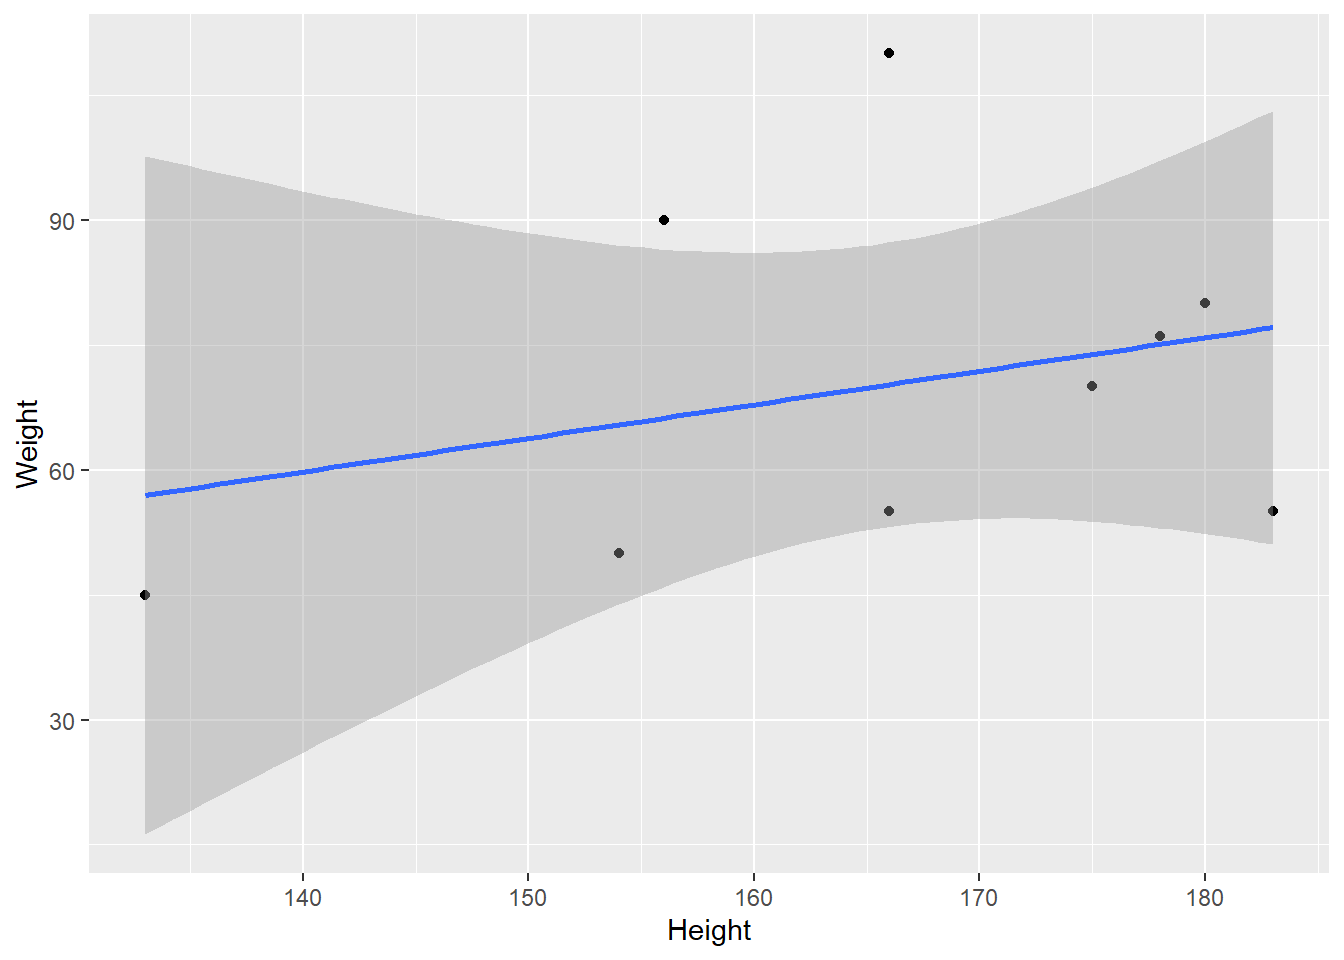
\includegraphics{Exercise-2_files/figure-pdf/unnamed-chunk-6-1.pdf}

}

\end{figure}

Predictors Skewness from Histogram:

\begin{itemize}
\tightlist
\item
  RI (Refractive Index): Right - Postive skewed
\item
  Na (Sodium): Right - Postive skewed
\item
  Mg (Magnesium):Left - Negative skewed
\item
  Al (Aluminum): Symmetrical, balanced
\item
  Si (Silicon): Left - Negatively skewed
\item
  K (Potassium): Left - Negative skewed
\item
  Ca (Calcium): Symmetrical, balanced
\item
  Ba (Barium): Non symmetrical
\item
  Fe (Iron): Non symmetrical
\end{itemize}

\textbf{Conclusion (Predictors):}

We can determine from the observations (Boxplot and Histograms), all but
one showed outliers with extreme values. Most of these predictors where
either skewed to the left (negative) or to the right (positive). All
this to say that we need to consider the outliers and the distribution
charactertics going forward.

\begin{enumerate}
\def\labelenumi{\alph{enumi})}
\setcounter{enumi}{2}
\tightlist
\item
  Are there any relevant transformations of one or more predictors that
  might improve the classification model? Show all the work!
\end{enumerate}

\begin{Shaded}
\begin{Highlighting}[]
\NormalTok{Glass\_transformed }\OtherTok{\textless{}{-}}\NormalTok{ Glass}
\NormalTok{Glass\_transformed[] }\OtherTok{\textless{}{-}} \FunctionTok{lapply}\NormalTok{(Glass\_transformed, }\ControlFlowTok{function}\NormalTok{(x) }\ControlFlowTok{if}\NormalTok{ (}\FunctionTok{is.numeric}\NormalTok{(x)) }\FunctionTok{log}\NormalTok{(x }\SpecialCharTok{+} \DecValTok{1}\NormalTok{) }\ControlFlowTok{else}\NormalTok{ x)}
\FunctionTok{names}\NormalTok{(Glass\_transformed)[}\FunctionTok{names}\NormalTok{(Glass\_transformed) }\SpecialCharTok{!=} \StringTok{"Type"}\NormalTok{] }\OtherTok{\textless{}{-}} \FunctionTok{paste0}\NormalTok{(}\StringTok{"log\_"}\NormalTok{, }\FunctionTok{names}\NormalTok{(Glass\_transformed)[}\FunctionTok{names}\NormalTok{(Glass\_transformed) }\SpecialCharTok{!=} \StringTok{"Type"}\NormalTok{])}

\NormalTok{Glass\_sqrt\_transformed }\OtherTok{\textless{}{-}}\NormalTok{ Glass}
\NormalTok{Glass\_sqrt\_transformed[] }\OtherTok{\textless{}{-}} \FunctionTok{lapply}\NormalTok{(Glass\_sqrt\_transformed, }\ControlFlowTok{function}\NormalTok{(x) }\ControlFlowTok{if}\NormalTok{ (}\FunctionTok{is.numeric}\NormalTok{(x)) }\FunctionTok{sqrt}\NormalTok{(x) }\ControlFlowTok{else}\NormalTok{ x)}
\FunctionTok{names}\NormalTok{(Glass\_sqrt\_transformed)[}\FunctionTok{names}\NormalTok{(Glass\_sqrt\_transformed) }\SpecialCharTok{!=} \StringTok{"Type"}\NormalTok{] }\OtherTok{\textless{}{-}} \FunctionTok{paste0}\NormalTok{(}\StringTok{"sqrt\_"}\NormalTok{, }\FunctionTok{names}\NormalTok{(Glass\_sqrt\_transformed)[}\FunctionTok{names}\NormalTok{(Glass\_sqrt\_transformed) }\SpecialCharTok{!=} \StringTok{"Type"}\NormalTok{])}

\NormalTok{Glass\_all\_transformed }\OtherTok{\textless{}{-}} \FunctionTok{cbind}\NormalTok{(Glass\_transformed, Glass\_sqrt\_transformed[,}\SpecialCharTok{{-}}\FunctionTok{which}\NormalTok{(}\FunctionTok{names}\NormalTok{(Glass\_sqrt\_transformed) }\SpecialCharTok{==} \StringTok{"Type"}\NormalTok{)])}

\NormalTok{log\_histograms }\OtherTok{\textless{}{-}} \FunctionTok{lapply}\NormalTok{(}\FunctionTok{names}\NormalTok{(Glass\_transformed)[}\DecValTok{1}\SpecialCharTok{:}\DecValTok{9}\NormalTok{], }\ControlFlowTok{function}\NormalTok{(var) \{}
  \FunctionTok{ggplot}\NormalTok{(Glass\_transformed, }\FunctionTok{aes\_string}\NormalTok{(}\AttributeTok{x =}\NormalTok{ var)) }\SpecialCharTok{+} 
    \FunctionTok{geom\_histogram}\NormalTok{(}\AttributeTok{bins =} \DecValTok{30}\NormalTok{) }\SpecialCharTok{+} 
    \FunctionTok{ggtitle}\NormalTok{(}\FunctionTok{paste}\NormalTok{(}\StringTok{"Histogram of"}\NormalTok{, var)) }\SpecialCharTok{+} 
    \FunctionTok{theme\_minimal}\NormalTok{() }\SpecialCharTok{+}
    \FunctionTok{theme\_classic}\NormalTok{()\})}

\NormalTok{sqrt\_histograms }\OtherTok{\textless{}{-}} \FunctionTok{lapply}\NormalTok{(}\FunctionTok{names}\NormalTok{(Glass\_sqrt\_transformed)[}\DecValTok{1}\SpecialCharTok{:}\DecValTok{9}\NormalTok{], }\ControlFlowTok{function}\NormalTok{(var) \{}
  \FunctionTok{ggplot}\NormalTok{(Glass\_sqrt\_transformed, }\FunctionTok{aes\_string}\NormalTok{(}\AttributeTok{x =}\NormalTok{ var)) }\SpecialCharTok{+} 
    \FunctionTok{geom\_histogram}\NormalTok{(}\AttributeTok{bins =} \DecValTok{30}\NormalTok{) }\SpecialCharTok{+} 
    \FunctionTok{ggtitle}\NormalTok{(}\FunctionTok{paste}\NormalTok{(}\StringTok{"Histogram of"}\NormalTok{, var)) }\SpecialCharTok{+} 
    \FunctionTok{theme\_minimal}\NormalTok{() }\SpecialCharTok{+}
    \FunctionTok{theme\_classic}\NormalTok{()\})}

\NormalTok{histogram\_combined }\OtherTok{\textless{}{-}} \FunctionTok{do.call}\NormalTok{(grid.arrange, }\FunctionTok{c}\NormalTok{(histograms, }\AttributeTok{ncol =} \DecValTok{3}\NormalTok{))}
\end{Highlighting}
\end{Shaded}

\begin{figure}[H]

{\centering 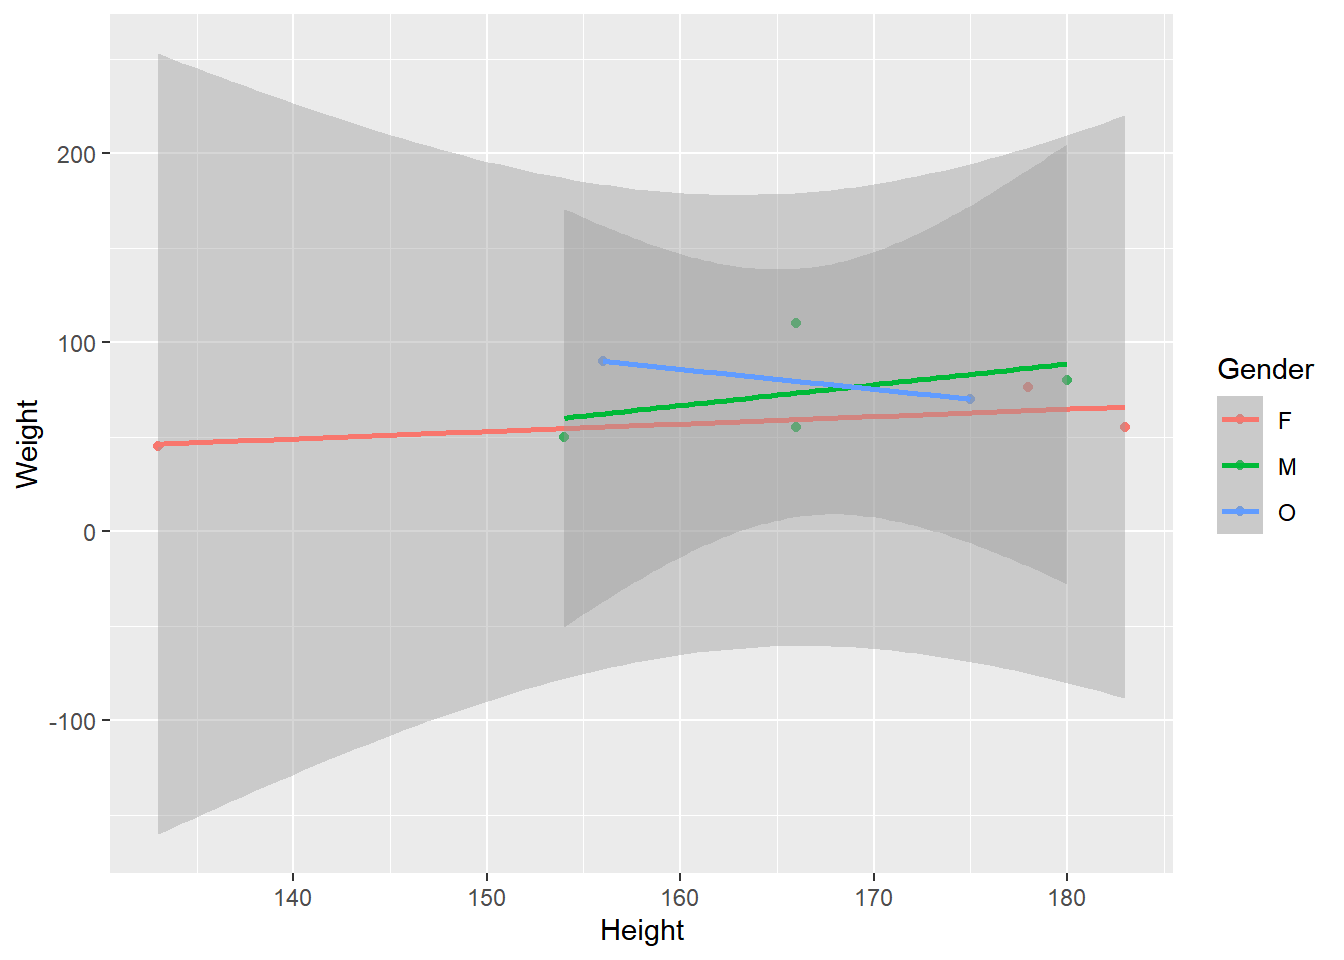
\includegraphics{Exercise-2_files/figure-pdf/unnamed-chunk-7-1.pdf}

}

\end{figure}

\begin{Shaded}
\begin{Highlighting}[]
\NormalTok{log\_histogram\_combined }\OtherTok{\textless{}{-}} \FunctionTok{do.call}\NormalTok{(grid.arrange, }\FunctionTok{c}\NormalTok{(log\_histograms, }\AttributeTok{ncol =} \DecValTok{3}\NormalTok{))}
\end{Highlighting}
\end{Shaded}

\begin{figure}[H]

{\centering 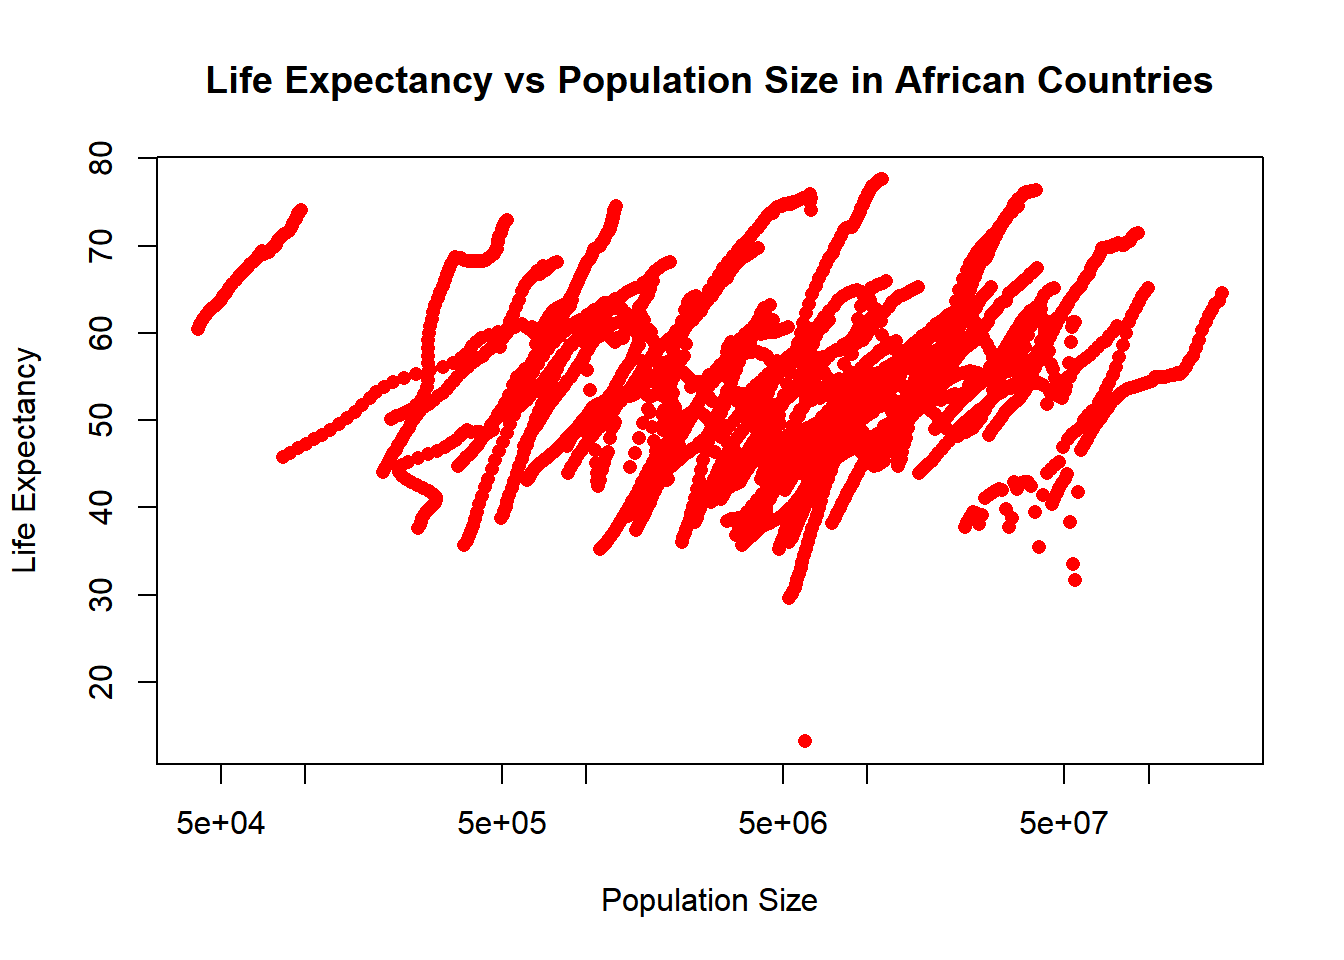
\includegraphics{Exercise-2_files/figure-pdf/unnamed-chunk-7-2.pdf}

}

\end{figure}

\begin{Shaded}
\begin{Highlighting}[]
\NormalTok{sqrt\_histogram\_combined }\OtherTok{\textless{}{-}} \FunctionTok{do.call}\NormalTok{(grid.arrange, }\FunctionTok{c}\NormalTok{(sqrt\_histograms, }\AttributeTok{ncol =} \DecValTok{3}\NormalTok{))}
\end{Highlighting}
\end{Shaded}

\begin{figure}[H]

{\centering \includegraphics{Exercise-2_files/figure-pdf/unnamed-chunk-7-3.pdf}

}

\end{figure}

\begin{Shaded}
\begin{Highlighting}[]
\FunctionTok{set.seed}\NormalTok{(}\DecValTok{123}\NormalTok{)}
\NormalTok{trainIndex }\OtherTok{\textless{}{-}} \FunctionTok{createDataPartition}\NormalTok{(Glass}\SpecialCharTok{$}\NormalTok{Type, }\AttributeTok{p =} \FloatTok{0.8}\NormalTok{, }\AttributeTok{list =} \ConstantTok{FALSE}\NormalTok{)}
\NormalTok{GlassTrain }\OtherTok{\textless{}{-}}\NormalTok{ Glass\_all\_transformed[trainIndex, ]}
\NormalTok{GlassTest }\OtherTok{\textless{}{-}}\NormalTok{ Glass\_all\_transformed[}\SpecialCharTok{{-}}\NormalTok{trainIndex, ]}

\NormalTok{model\_transformed }\OtherTok{\textless{}{-}} \FunctionTok{train}\NormalTok{(Type }\SpecialCharTok{\textasciitilde{}}\NormalTok{ ., }\AttributeTok{data =}\NormalTok{ GlassTrain, }\AttributeTok{method =} \StringTok{\textquotesingle{}rpart\textquotesingle{}}\NormalTok{)}


\NormalTok{pred\_transformed }\OtherTok{\textless{}{-}} \FunctionTok{predict}\NormalTok{(model\_transformed, }\AttributeTok{newdata =}\NormalTok{ GlassTest)}


\NormalTok{cm\_transformed }\OtherTok{\textless{}{-}} \FunctionTok{confusionMatrix}\NormalTok{(pred\_transformed, GlassTest}\SpecialCharTok{$}\NormalTok{Type)}

\FunctionTok{cat}\NormalTok{(}\StringTok{"Transformed Model Performance:}\SpecialCharTok{\textbackslash{}n}\StringTok{"}\NormalTok{)}
\end{Highlighting}
\end{Shaded}

\begin{verbatim}
Transformed Model Performance:
\end{verbatim}

\begin{Shaded}
\begin{Highlighting}[]
\FunctionTok{print}\NormalTok{(cm\_transformed)}
\end{Highlighting}
\end{Shaded}

\begin{verbatim}
Confusion Matrix and Statistics

          Reference
Prediction  1  2  3  5  6  7
         1 11  8  2  0  0  0
         2  3  7  1  1  1  0
         3  0  0  0  0  0  0
         5  0  0  0  0  0  0
         6  0  0  0  0  0  0
         7  0  0  0  1  0  5

Overall Statistics
                                          
               Accuracy : 0.575           
                 95% CI : (0.4089, 0.7296)
    No Information Rate : 0.375           
    P-Value [Acc > NIR] : 0.008001        
                                          
                  Kappa : 0.371           
                                          
 Mcnemar's Test P-Value : NA              

Statistics by Class:

                     Class: 1 Class: 2 Class: 3 Class: 5 Class: 6 Class: 7
Sensitivity            0.7857   0.4667    0.000     0.00    0.000   1.0000
Specificity            0.6154   0.7600    1.000     1.00    1.000   0.9714
Pos Pred Value         0.5238   0.5385      NaN      NaN      NaN   0.8333
Neg Pred Value         0.8421   0.7037    0.925     0.95    0.975   1.0000
Prevalence             0.3500   0.3750    0.075     0.05    0.025   0.1250
Detection Rate         0.2750   0.1750    0.000     0.00    0.000   0.1250
Detection Prevalence   0.5250   0.3250    0.000     0.00    0.000   0.1500
Balanced Accuracy      0.7005   0.6133    0.500     0.50    0.500   0.9857
\end{verbatim}

After I applied the transformation and achieved accuracy of 57.5\%, and
the Kappa is 0.371. We can say there is a level of agreement between the
variables. Now looking at the classes that were observed we can see that
class 1 and 2 are strong in their classification while the rest need
improvement. Maybe if we refine our focus on the variblae we observe we
can improve out accurancy.

\begin{enumerate}
\def\labelenumi{\alph{enumi})}
\setcounter{enumi}{3}
\tightlist
\item
  Fit SVM model (You may refer to Chapter 4 material for details) using
  the following R codes: (This code will be discussed in detail in the
  following chapters)
\end{enumerate}

\begin{Shaded}
\begin{Highlighting}[]
\FunctionTok{set.seed}\NormalTok{(}\DecValTok{231}\NormalTok{) }
\NormalTok{sigDist }\OtherTok{\textless{}{-}} \FunctionTok{sigest}\NormalTok{(Type}\SpecialCharTok{\textasciitilde{}}\NormalTok{ ., }\AttributeTok{data =}\NormalTok{ Glass, }\AttributeTok{frac =} \DecValTok{1}\NormalTok{)}
\NormalTok{sigDist }
\end{Highlighting}
\end{Shaded}

\begin{verbatim}
       90%        50%        10% 
0.03407935 0.11297847 0.62767315 
\end{verbatim}

\begin{Shaded}
\begin{Highlighting}[]
\NormalTok{svmTuneGrid }\OtherTok{\textless{}{-}} \FunctionTok{data.frame}\NormalTok{(}\AttributeTok{sigma =} \FunctionTok{as.vector}\NormalTok{(sigDist)[}\DecValTok{1}\NormalTok{], }\AttributeTok{C =} \DecValTok{2}\SpecialCharTok{\^{}}\NormalTok{(}\SpecialCharTok{{-}}\DecValTok{2}\SpecialCharTok{:}\DecValTok{10}\NormalTok{)) }
\NormalTok{svmTuneGrid }
\end{Highlighting}
\end{Shaded}

\begin{verbatim}
        sigma       C
1  0.03407935    0.25
2  0.03407935    0.50
3  0.03407935    1.00
4  0.03407935    2.00
5  0.03407935    4.00
6  0.03407935    8.00
7  0.03407935   16.00
8  0.03407935   32.00
9  0.03407935   64.00
10 0.03407935  128.00
11 0.03407935  256.00
12 0.03407935  512.00
13 0.03407935 1024.00
\end{verbatim}

\begin{Shaded}
\begin{Highlighting}[]
\FunctionTok{set.seed}\NormalTok{(}\DecValTok{231}\NormalTok{)}

\NormalTok{sigDist }\OtherTok{\textless{}{-}} \FunctionTok{sigest}\NormalTok{(Type }\SpecialCharTok{\textasciitilde{}}\NormalTok{ ., }\AttributeTok{data =}\NormalTok{ Glass, }\AttributeTok{frac =} \DecValTok{1}\NormalTok{)}

\NormalTok{svmTuneGrid }\OtherTok{\textless{}{-}} \FunctionTok{data.frame}\NormalTok{(}\AttributeTok{sigma =} \FunctionTok{as.vector}\NormalTok{(sigDist)[}\DecValTok{1}\NormalTok{], }\AttributeTok{C =} \DecValTok{2}\SpecialCharTok{\^{}}\NormalTok{(}\SpecialCharTok{{-}}\DecValTok{2}\SpecialCharTok{:}\DecValTok{10}\NormalTok{))}

\NormalTok{svmModel }\OtherTok{\textless{}{-}} \FunctionTok{ksvm}\NormalTok{(Type }\SpecialCharTok{\textasciitilde{}}\NormalTok{ ., }\AttributeTok{data =}\NormalTok{ Glass, }\AttributeTok{type =} \StringTok{"C{-}svc"}\NormalTok{, }\AttributeTok{kernel =} \StringTok{"rbfdot"}\NormalTok{, }\AttributeTok{kpar =} \FunctionTok{list}\NormalTok{(}\AttributeTok{sigma =} \FunctionTok{as.vector}\NormalTok{(sigDist)[}\DecValTok{1}\NormalTok{]), }\AttributeTok{C =} \DecValTok{2}\SpecialCharTok{\^{}}\NormalTok{(}\SpecialCharTok{{-}}\DecValTok{2}\SpecialCharTok{:}\DecValTok{10}\NormalTok{))}

\FunctionTok{print}\NormalTok{(svmModel)}
\end{Highlighting}
\end{Shaded}

\begin{verbatim}
Support Vector Machine object of class "ksvm" 

SV type: C-svc  (classification) 
 parameter : cost C = 0.25 
  parameter : cost C = 0.5 
  parameter : cost C = 1 
  parameter : cost C = 2 
  parameter : cost C = 4 
  parameter : cost C = 8 
  parameter : cost C = 16 
  parameter : cost C = 32 
  parameter : cost C = 64 
  parameter : cost C = 128 
  parameter : cost C = 256 
  parameter : cost C = 512 
  parameter : cost C = 1024 

Gaussian Radial Basis kernel function. 
 Hyperparameter : sigma =  0.0340793487610772 

Number of Support Vectors : 205 

Objective Function Value : -30.8971 -8.4786 -4.7642 -3.9839 -4.8778 -8.4545 -6.0399 -4.2908 -6.4624 -4.3643 -3.8975 -4.5021 -3.8506 -4.9211 -4.0869 
Training error : 0.439252 
\end{verbatim}

\begin{Shaded}
\begin{Highlighting}[]
\FunctionTok{set.seed}\NormalTok{(}\DecValTok{1056}\NormalTok{)}
\CommentTok{\# Fit SVM model using 10{-}fold cross{-}validation}
\NormalTok{svmFit }\OtherTok{\textless{}{-}} \FunctionTok{train}\NormalTok{(Type }\SpecialCharTok{\textasciitilde{}}\NormalTok{ .,}
                \AttributeTok{data =}\NormalTok{ Glass, }\AttributeTok{method =} \StringTok{"svmRadial"}\NormalTok{,}
                \AttributeTok{preProcess =} \FunctionTok{c}\NormalTok{(}\StringTok{"center"}\NormalTok{, }\StringTok{"scale"}\NormalTok{),}
                \AttributeTok{tuneGrid =}\NormalTok{ svmTuneGrid,}
                \AttributeTok{trControl =} \FunctionTok{trainControl}\NormalTok{(}\AttributeTok{method =} \StringTok{"repeatedcv"}\NormalTok{, }\AttributeTok{repeats =} \DecValTok{5}\NormalTok{))}


\FunctionTok{plot}\NormalTok{(svmFit, }\AttributeTok{scales =} \FunctionTok{list}\NormalTok{(}\AttributeTok{x =} \FunctionTok{list}\NormalTok{(}\AttributeTok{log =} \DecValTok{2}\NormalTok{)))}
\end{Highlighting}
\end{Shaded}

\begin{figure}[H]

{\centering 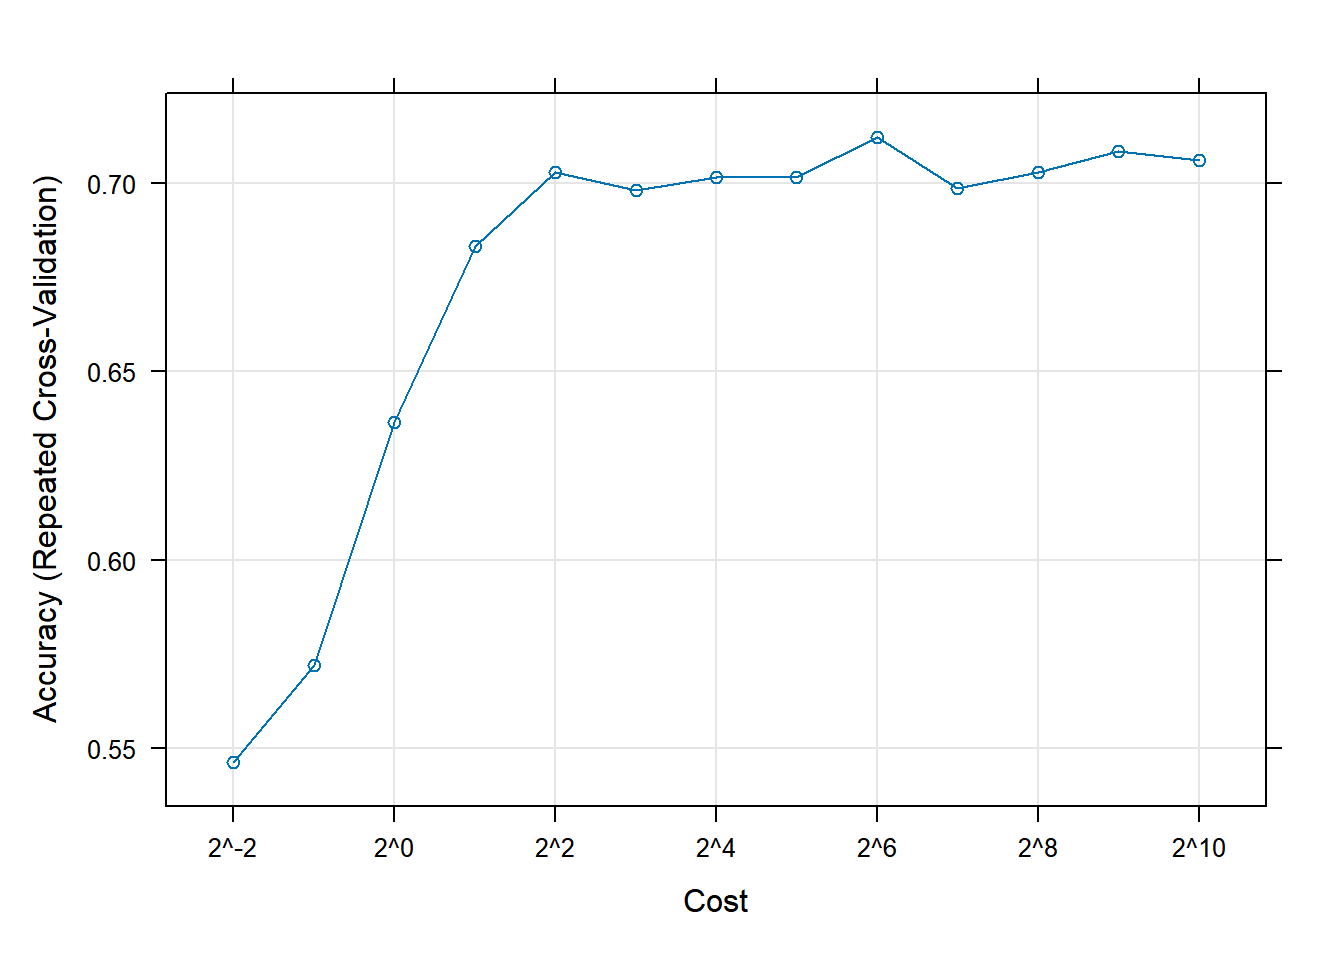
\includegraphics{Exercise-2_files/figure-pdf/train-svm-model-1.pdf}

}

\end{figure}



\end{document}
